% Autogenerated translation of README.md by Texpad
% To stop this file being overwritten during the typeset process, please move or remove this header

\documentclass[12pt]{book}
\usepackage{graphicx}
\usepackage{fontspec}
\usepackage[utf8]{inputenc}
\usepackage[a4paper,left=.5in,right=.5in,top=.3in,bottom=0.3in]{geometry}
\setlength\parindent{0pt}
\setlength{\parskip}{\baselineskip}
\setmainfont{Helvetica Neue}
\usepackage{hyperref}
\pagestyle{plain}
\begin{document}

\chapter*{Elate Theme}

Elate is a one page portfolio for freelancers, designers, developers and even agencies based on the \href{//freehtml5.co/elate-free-html5-bootstrap-template/}{original html5 theme}. 
This Hugo theme features several content sections, a contact form, a responsive portfolio grid with hover effects, a smooth parallax and animation effect on sections. Its packed with 4 ready to use styles.

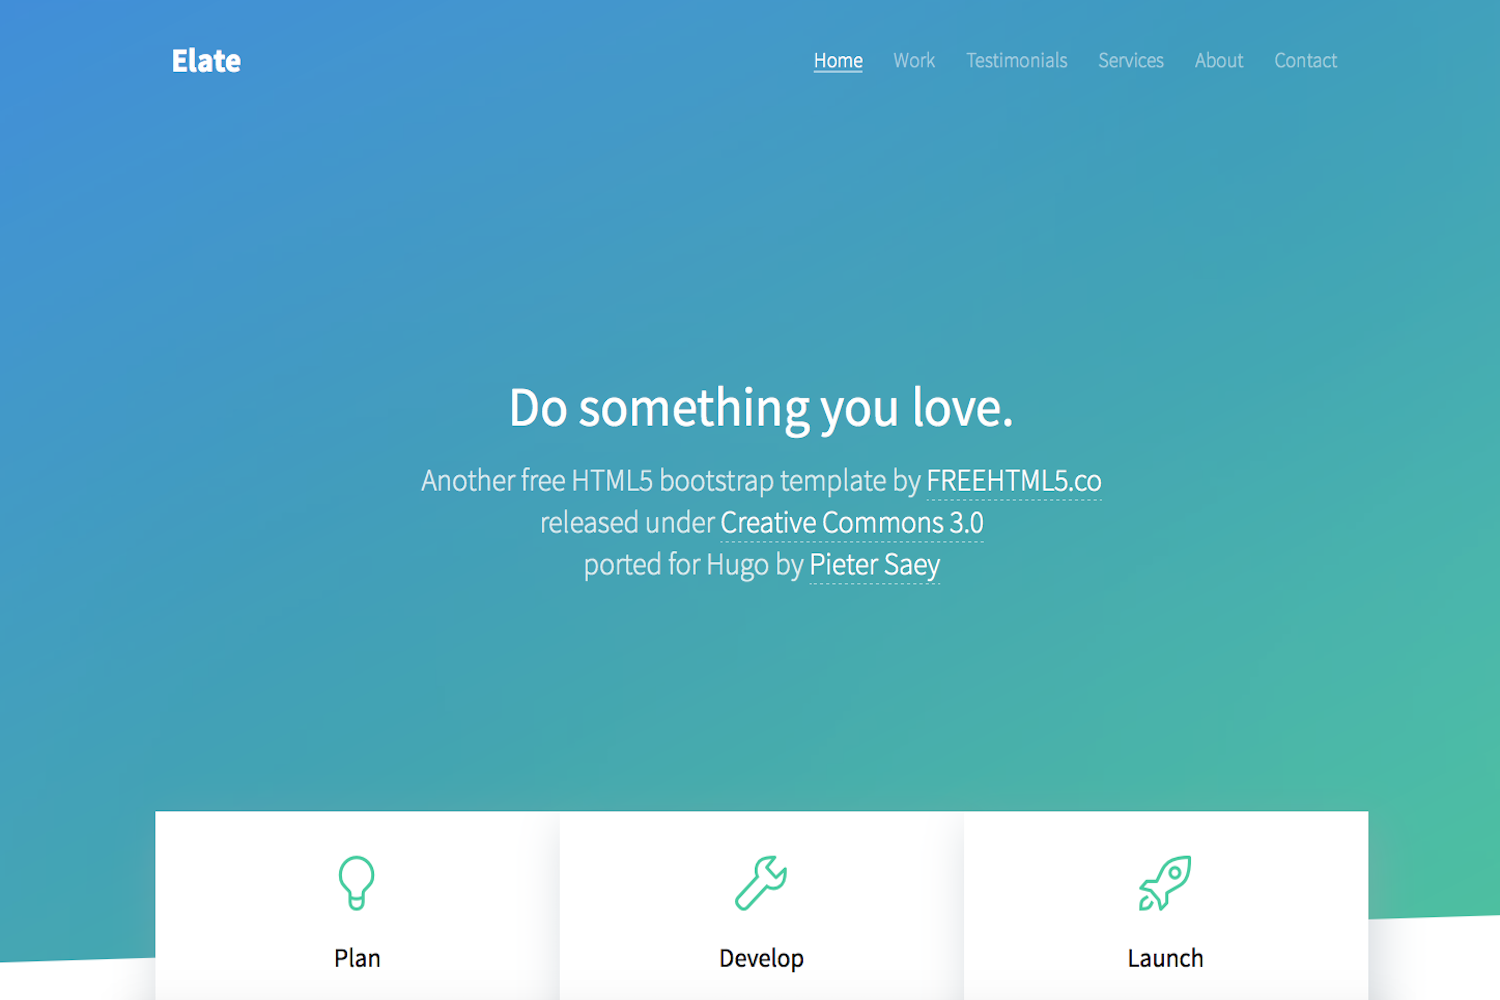
\includegraphics{https://raw.githubusercontent.com/saey55/hugo-elate-theme/master/images/screenshot.png}

\section*{Installation}

Inside the folder of your Hugo site run:

\begin{verbatim}
$ cd themes
$ git clone https://github.com/saey55/hugo-elate-theme
\end{verbatim}

For more information read the official \href{//gohugo.io/overview/installing/}{setup guide} of Hugo.

\section*{Getting started}

After installing the Elate Theme successfully it requires a just a few more steps to get your site running.

\subsection*{The config file}

Take a look inside the \href{//github.com/saey55/hugo-elate-theme/tree/master/exampleSite}{\texttt{exampleSite}} folder of this theme. You'll find a file called \href{//github.com/saey55/hugo-elate-theme/blob/master/exampleSite/config.toml}{\texttt{config.toml}}. To use it, copy the \href{//github.com/saey55/hugo-elate-theme/blob/master/exampleSite/config.toml}{\texttt{config.toml}} in the root folder of your Hugo site. Feel free to change the strings in this theme.

\subsection*{Make the contact form working}

Since this page will be static, you can use \href{//formspree.io/}{formspree.io} as proxy to send the actual email. Each month, visitors can send you up to one thousand emails without incurring extra charges. Begin the setup by following the steps below:

\begin{enumerate}
\item Enter your email address under 'email' in the \href{//github.com/saey55/hugo-elate-theme/blob/master/exampleSite/config.toml}{\texttt{config.toml}}
\item Enable form by setting \texttt{enable} to \texttt{true} in contact settings
\item Upload the generated site to your server
\item Send a dummy email yourself to confirm your account
\item Click the confirm link in the email from \href{//formspree.io/}{formspree.io}
\item You're done. Happy mailing!
\end{enumerate}

\subsection*{Nearly finished}

In order to see your site in action, run Hugo's built-in local server. 

\begin{verbatim}
$ hugo server
\end{verbatim}

Now enter \href{http://localhost:1313/}{\texttt{localhost:1313}} in the address bar of your browser.

\section*{Contributing}

Did you find a bug or have an idea for a new feature? Feel free to use the \href{//github.com/saey55/hugo-elate-theme/issues}{issue tracker} to let me know. Or make directly a \href{//github.com/saey55/hugo-elate-theme/pulls}{pull request}.

\section*{License}

This theme is released under The MIT License (MIT). For more information read the \href{//github.com/saey55/hugo-elate-theme/blob/master/LICENSE.md}{License}.

\section*{Acknowledgements}

Thanks to 

\begin{itemize}
\item \href{//freehtml5.co}{freehtml5.co} for creating this theme
\item \href{//github.com/spf13}{Steve Francia} for creating Hugo and the awesome community around the project.
\end{itemize}

\end{document}
